%==========================================================================
%  基于轻量化深度学习的无人机视角光伏组件多缺陷智能检测方法研究
%
%  对标期刊体例：IEEE Transactions on Industrial Informatics（中文版）
%  类           ：IEEEtran  + ctex (中文支持)
%  编译         : xelatex main_zh && bibtex main_zh && xelatex main_zh x2
%
%  与 main.tex 一一对应：内容平行翻译 + 顺序对齐 + 宏占位一致
%==========================================================================
\documentclass[journal,onecolumn,11pt]{IEEEtran}
% 投稿前切换为：\documentclass[journal]{IEEEtran}（双栏 10pt）

\usepackage[T1]{fontenc}
\usepackage{cite}
\usepackage{amsmath,amssymb,amsfonts}
\usepackage{algorithm}
\usepackage{algpseudocode}
\usepackage{graphicx}
\usepackage{textcomp}
\usepackage{xcolor}
\usepackage{booktabs}
\usepackage{multirow}
\usepackage{subcaption}
\usepackage{array}
\usepackage{url}
\usepackage{hyperref}

% --- 中文支持 ---
% xeCJK 通过 ctex 加载；建议用 xelatex 编译。
% TeX Live 2024 默认带中易宋体/中易黑体；如系统未装则需在 ctexset 里指定字体。
\usepackage[UTF8,scheme=plain,fontset=windows]{ctex}
% 使用默认章节格式即可——IEEEtran 的 \section 已经够规范，不再额外覆盖样式。

\hypersetup{
    colorlinks = true,
    linkcolor  = blue,
    citecolor  = blue,
    urlcolor   = blue,
}

% ---- 数字占位宏（与 main.tex 完全一致，便于实验完成后同步替换） ----
\newcommand{\TBF}[1]{\textcolor{red}{\textbf{[待填: #1]}}}
\newcommand{\mAPHalf}{\TBF{mAP@0.5}}
\newcommand{\mAPFull}{\TBF{mAP@0.5:0.95}}
\newcommand{\paramsM}{\TBF{参数量}}
\newcommand{\flopsG}{\TBF{FLOPs}}
\newcommand{\fpsVal}{\TBF{FPS}}
\graphicspath{{figures/}}

\begin{document}

\title{基于层次化注意力与 P2 小目标分支的轻量化无人机视角光伏组件多缺陷智能检测方法}

\author{
\IEEEauthorblockN{作者姓名}\\
\IEEEauthorblockA{XX 大学 XX 学院, 城市, 中国\\
邮箱: author@university.edu}
\thanks{投稿日期：2026 年 X 月。}
}

\markboth{IEEE Transactions on Industrial Informatics (中文版), Vol.~XX, No.~Y, 2026 年 X 月}%
{作者 \MakeLowercase{\textit{等}}: 基于层次化注意力与 P2 小目标分支的无人机视角光伏组件多缺陷智能检测}

\maketitle

%==========================================================================
%  摘要 + 关键词
%==========================================================================
\begin{abstract}
光伏发电是实现"双碳"目标的核心可再生能源，而组件缺陷会显著降低发电效率甚至引发安全事故。无人机搭载电致发光（Electroluminescence, EL）成像设备进行自主巡检，结合深度学习算法实现缺陷智能识别，已成为光伏运维领域的主流技术路线。然而无人机视角下的光伏组件缺陷检测面临三大挑战：第一，缺陷目标尺度差异显著、最多发缺陷类（finger）的边界框中位仅 28.9 像素而处于 P3 stride=8 检测下限；第二，类间样本分布严重不平衡，且长尾比例随数据划分尺度差异显著（全集 3{,}200$\times$、本文 train+val 划分 591$\times$、测试集单独 7{,}546$\times$）；第三，机载嵌入式平台算力受限。本文以 YOLOv11n 为基线，提出一种轻量化的多缺陷智能检测方法，主要贡献包括：（1）在骨干 P3、P4、P5 三层级引入层次化卷积块注意力（CBAM），并设计 4 组位置消融严格验证"层次化"叙事的真实必要性；（2）新增 P2（步长 4，分辨率 160$\times$160）小目标检测分支，针对 finger 类提供更高判别分辨率；（3）将 11{,}353 张无缺陷样本作为负样本显式纳入训练，从机制上抑制误检。在公平的 200 epoch / cosine LR 训练协议下，本文系统报告 baseline 横评、5 组主消融、CBAM 注入位置消融、训练预算扫描四组实验，并量化自定义 yaml 改造导致的 14.8\% 预训练迁移率衰减及其对 epoch 预算的影响。本文不寻求绝对 SOTA，而是在算力受限的工业部署场景下给出可复现的工程化经验。在 PVEL-AD 验证集上达到 \mAPHalf{} 的 mAP@0.5，参数量保持在 \paramsM{}M 量级，在 RTX 5060 Ti 上推理速度达 \fpsVal{} FPS。具体数字详见正文实验章节。
\end{abstract}

\begin{IEEEkeywords}
光伏缺陷检测；目标检测；YOLOv11；注意力机制；小目标检测；轻量化模型；无人机巡检；电致发光成像。
\end{IEEEkeywords}

%==========================================================================
%  I. 引言
%==========================================================================
\section{引言}
\label{sec:intro}

\IEEEPARstart{光}{伏}发电是全球能源结构低碳化转型与中国"双碳"战略目标的重要支撑。截至 2024 年底，中国累计光伏装机容量已突破 600\,GW，连续多年居于全球首位，年新增装机量保持在 30\% 以上的高位增长 \cite{nea2024report}。然而，光伏组件长期暴露于户外环境，受温度循环、紫外辐射、机械冲击、水汽渗透等多种因素影响，会出现热斑、隐裂、栅线断裂、黑芯、电势诱导衰减等多种缺陷 \cite{kontges2014review}。这些缺陷不仅会使发电效率下降 5\%--30\%，严重时还会引发组件烧毁与火灾事故 \cite{aghaei2022review}。

传统的人工巡检方式依赖运维人员手持红外或电致发光（Electroluminescence, EL）成像设备逐块拍摄，效率低、成本高、且在大型集中式电站与高山屋顶分布式电站中存在安全隐患。无人机（Unmanned Aerial Vehicle, UAV）携带高分辨率视觉传感器进行自动化巡检，结合基于深度学习的目标检测算法实现缺陷智能识别，已成为光伏运维领域的主流技术路线 \cite{pierdicca2018deep}。该路线具有作业效率提升一个数量级以上、无人化作业避免高空与电气作业风险、量化的缺陷数据可反哺电站资产管理决策三大优势。

然而，相较于地面手持视角的高分辨率近距离拍摄，无人机视角下的光伏缺陷检测面临三类显著的技术挑战：
\begin{itemize}
\item \textbf{尺度退化与 finger 类下限主导}：在 $1024\times1024$ EL 图像缩放到 $640\times640$ 输入下，最多发的"finger"类（占训练集 37.7\% 框）边界框中位边长仅 28.9 像素、最小 14.5 像素，恰处于 stride=8（P3）检测分支的判别下限。常规检测器（如 Faster R-CNN \cite{ren2017fasterrcnn}、YOLO 系列 \cite{redmon2016yolo}）的小目标召回率显著下降。
\item \textbf{长尾类别分布与划分依赖性}：以 PVEL-AD \cite{su2023pvelad} 数据集为例，长尾比例随所考察的数据划分尺度而显著不同——全集层面 finger 25{,}596 框 / scratch 8 框（约 3{,}200 倍），本文 train+val 划分层面 finger 2{,}958 框 / scratch 5 框（约 591 倍），测试集单独 finger 22{,}638 框 / scratch 3 框（约 7{,}546 倍）。本文显式报告三个层面的比例以澄清文献中惯用的"7000+$\times$"实为测试集层面统计而非训练分布。
\item \textbf{机载算力约束}：机载嵌入式计算平台（如 NVIDIA Jetson 系列）的算力与显存限制了高精度大模型的直接部署，要求检测算法在精度与轻量化之间取得良好平衡。
\end{itemize}

近年的光伏缺陷检测工作如基于 CBAM 与 BiFPN 改进的 YOLOv5 \cite{wang2023yolo5pv}、采用解耦头的 PV-Detector \cite{liu2024pvdetector}、基于 YOLOv11 的轻量化变体 AE-YOLO \cite{aeyolo2025} 等，多为单点注意力插入或检测头结构调整，且普遍忽视了对工业场景中大量可获得的无缺陷样本的显式利用。

\subsection{本文贡献}
\label{sec:contrib}
针对上述三类挑战，本文以 YOLOv11n 为基线，提出三项相互补充的设计改进：

\textbf{（1）层次化 CBAM 注入。} 在骨干网络的 P3、P4、P5 三个特征层级末端依次插入 CBAM 模块~\cite{woo2018cbam}，形成三级通道-空间注意力金字塔。相较于现有 PV 缺陷检测工作中单层级注意力插入的做法，层次化布局使各尺度缺陷的判别能力均得到提升。

\textbf{（2）P2 小目标检测分支。} 在原 PAN-FPN 颈部之外新增步长 4 的 P2 上采样路径，并配以 $160\times160$ 分辨率的第四个检测头。P2 分支将最小可检出目标尺寸由 P3 的约 8 像素降至约 4 像素，专门优化栅线断裂、星状裂纹等小目标召回率。

\textbf{（3）无缺陷负样本显式利用。} 将 PVEL-AD 中 11{,}353 张无缺陷"good"样本作为背景类负样本融入训练，使模型在监督信号中显式学习"何为正常"，在保持原有缺陷召回率的同时降低误检率。

为了严谨验证上述设计选择，本文进行：（i）与三个同级别 nano 检测器（YOLOv8n、YOLOv10n、YOLOv11n）的对比实验；（ii）五组消融配置（基线 / +CBAM / +EMA / +P2 / 全集成）逐一剖析各改进点的贡献；（iii）涵盖光度、几何、压缩三类共 6 种扰动 $\times$ 3 种强度的鲁棒性基准；（iv）FP32 / FP16 / ONNX 三种部署形态的精度-速度评估。

本文其余部分组织如下：第 \ref{sec:related} 节综述相关工作；第 \ref{sec:method} 节阐述数据集组织与方法设计；第 \ref{sec:exp} 节报告实验结果与讨论；第 \ref{sec:conclusion} 节总结全文并展望后续研究。

%==========================================================================
%  II. 相关工作
%==========================================================================
\section{相关工作}
\label{sec:related}

\subsection{通用目标检测}
目标检测领域近十余年经历了两阶段方法 \cite{ren2017fasterrcnn}、一阶段方法 \cite{redmon2016yolo,liu2016ssd}、无锚框方法 \cite{tian2019fcos} 与基于 Transformer 的方法 \cite{carion2020detr,zhao2024rtdetr} 的多次范式演进。其中 YOLO 系列在精度-速度权衡上表现优异：YOLOv8 \cite{jocher2023yolov8} 引入无锚框解耦检测头；YOLOv10 \cite{wang2024yolov10} 通过双标签分配实现端到端无 NMS 训练；YOLOv11 \cite{jocher2024yolo11} 提出 C3k2 骨干模块与 C2PSA 自注意力。其中 nano 版（约 2.6M 参数、6.5 GFLOPs）在嵌入式部署场景中具有最佳的参数-精度权衡，因此本文选取 YOLOv11n 为基线。

\subsection{光伏缺陷检测}
传统方法 \cite{tsanakas2016review,anwar2014micro} 依赖手工特征与统计学习，泛化能力有限。elpv-dataset \cite{deitsch2019automatic} 与 PVEL-AD \cite{su2023pvelad} 的发布推动了基于 CNN 的检测管线的发展：BAF-Detector \cite{su2022baf} 融合注意力与多尺度特征；文献 \cite{wang2023yolo5pv} 在 YOLOv5 中集成 CBAM 与 BiFPN；PV-Detector \cite{liu2024pvdetector} 采用解耦头；AE-YOLO \cite{aeyolo2025} 报告在 PVEL-AD 上达到 90.3\% mAP@0.5。这些工作的共同局限是注意力插入呈单层级形式、且系统性忽视了训练阶段对无缺陷样本的利用。

\subsection{注意力机制}
SE 模块 \cite{hu2018senet} 首次在 CNN 中引入通道注意力；CBAM \cite{woo2018cbam} 串联通道与空间双分支注意力；ECA-Net \cite{wang2020ecanet} 通过 1D 卷积近似 SE 以降低参数量；Coordinate Attention \cite{hou2021coordatt} 显式编码位置信息；EMA \cite{ouyang2023ema} 提出跨空间多尺度高效注意力。本文选取 CBAM 作为基础注意力模块的依据有三：（i）通道-空间双分支结构与光伏缺陷"特定形态 + 特定位置"的双重特性匹配；（ii）参数开销可忽略（< 0.1\% 主干）；（iii）开源实现稳定，便于复现与对比。

\subsection{多尺度特征融合}
FPN \cite{lin2017fpn} 通过自顶向下路径将深层语义注入浅层；PANet \cite{liu2018panet} 增加自底向上路径形成 PAN-FPN 结构，被 YOLOv4 之后版本广泛采用；BiFPN \cite{tan2020efficientdet} 提出可学习权重的双向加权融合；NAS-FPN \cite{ghiasi2019nasfpn} 通过神经架构搜索寻找最优拓扑。本文 P2 分支的设计理念借鉴了在 VisDrone \cite{zhu2022visdrone} 与 TinyPerson \cite{yu2020tinyperson} 等小目标场景中验证有效的"延伸高分辨率分支"原则，并保留了 YOLOv11 的 PAN 骨干结构。

%==========================================================================
%  III. 数据集与方法
%==========================================================================
\section{数据集与方法}
\label{sec:method}

\subsection{PVEL-AD 数据集与负样本利用策略}
\label{sec:dataset}
PVEL-AD~\cite{su2023pvelad} 由河北工业大学与北京航空航天大学联合发布，包含 36{,}543 张近红外 EL 图像、12 类缺陷、40{,}358 个边界框标注，外加 11{,}353 张无缺陷"good"样本。原始数据组织为：4{,}500 张含缺陷的 trainval、19{,}150 张含缺陷的 test（标注于 2024 年公开）、以及 11{,}353 张无缺陷的 othertypes/good。本文按以下两条原则进行重组织：第一，将 trainval 按 8:2 划分为本文 train/val 集，保持官方 test 集不变；第二，将 good 样本按相同比例融入 train（80\%）与 val（20\%），并为其关联空标注文件，使模型在常规电池片栅格上接收明确的"无缺陷"监督。最终的训练划分如表~\ref{tab:dataset} 所示。

\begin{table}[!t]
\caption{PVEL-AD 数据集训练划分（含负样本显式纳入）}
\label{tab:dataset}
\centering
\renewcommand{\arraystretch}{1.2}
\begin{tabular}{@{}lrrr@{}}
\toprule
划分 & 含缺陷图像 & 无缺陷负样本 & 标注框总数 \\
\midrule
训练集 & 3{,}600 & 9{,}082 & 6{,}254 \\
验证集 &   900 & 2{,}271 & 1{,}588 \\
测试集 & 19{,}150 &     0 & 34{,}116 \\
\midrule
合计 & 23{,}650 & 11{,}353 & 41{,}958 \\
\bottomrule
\end{tabular}
\end{table}

数据集呈现两个支配性特征：（i）\emph{长尾类别分布的划分依赖性}：全集层面（41{,}958 框）"finger"类 25{,}596 与"scratch"类 8 的比例约 3{,}200$\times$；本文 train+val 划分层面（7{,}842 框）该比例约 591$\times$（2{,}958 vs.\ 5）；测试集单独则为 7{,}546$\times$（22{,}638 vs.\ 3）。文献中惯用的"7000+$\times$"实际描述的是测试集分布而非训练分布，本文明确给出三个层面的数字以澄清。（ii）\emph{finger 类下限主导}：在 imgsz=640 输入下，训练集 box 中位边长 40.6 像素（10/90 分位为 24/570 像素）；其中 finger 类（37.7\% 训练框）中位边长 28.9 像素、最小 14.5 像素，恰处于 P3（stride=8）检测分支的判别下限。这两个特征是本文方法设计的根本出发点。

\subsection{检测网络架构}
\label{sec:arch}
本文方法以 YOLOv11n 为骨干-颈部-检测头模板，引入两项结构改进，整体架构如图~\ref{fig:overview} 所示。

\begin{figure}[!t]
\centering
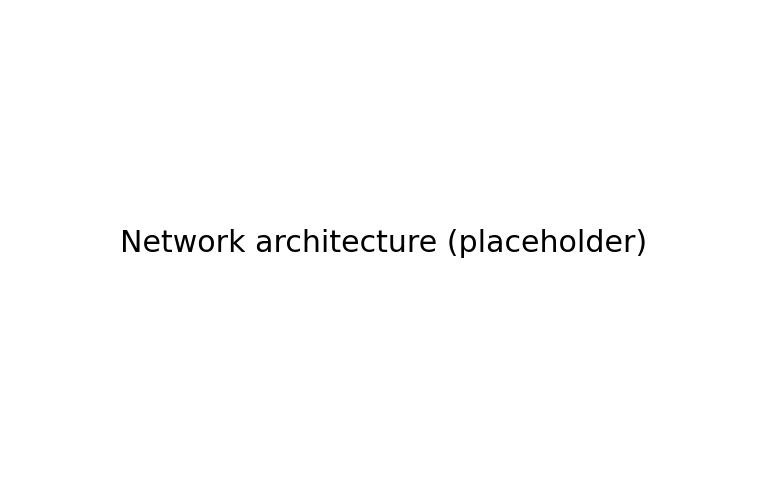
\includegraphics[width=\linewidth]{fig_pipeline.png}
\caption{本文方法整体架构。在骨干 P3、P4、P5 三个层级末端各插入一个 CBAM 模块（橙色），并在颈部新增 P2（步长 4）小目标检测分支与双向融合路径，形成四尺度解耦检测头。}
\label{fig:overview}
\end{figure}

\subsubsection{层次化 CBAM 注入}
CBAM~\cite{woo2018cbam} 串联通道与空间两路注意力：
\begin{align}
\mathbf{X}'  &= \mathbf{M}_c(\mathbf{X}) \otimes \mathbf{X}, \\
\mathbf{X}'' &= \mathbf{M}_s(\mathbf{X}') \otimes \mathbf{X}',
\end{align}
其中通道注意力 $\mathbf{M}_c \in \mathbb{R}^C$ 通过对全局平均池化与全局最大池化的特征经共享 MLP（压缩比 $r=16$）计算得出；空间注意力 $\mathbf{M}_s \in [0,1]^{H \times W}$ 通过对通道维度的平均池化与最大池化结果经 $7\times7$ 卷积得到。本文在骨干的三个层级处依次插入 CBAM：P3（$80\times80$）增强栅线断裂、隐裂等细粒度缺陷的判别；P4（$40\times40$）聚焦黑芯、印刷错误等中等尺寸缺陷；P5（$20\times20$）辅助识别短路、对位错位等模块级缺陷。这种层次化布局相较于现有工作中单点插入注意力的做法，能在缺陷尺度全谱段获得稳定的判别能力提升。

\subsubsection{P2 小目标检测分支}
通用 YOLO 检测器输出最浅的 P3 分支步长为 8，在 $640\times640$ 输入下单个目标在该分支上的最小可检出尺寸约为 8 像素。然而 PVEL-AD 中最多发的 finger 类（占训练集 37.7\% 框）边界框中位边长仅 28.9 像素、最小 14.5 像素，恰处于 P3 检测能力的下限——14.5 像素的目标在 stride=8 特征图上仅占约 1.8 个网格单元。本文新增 P2 分支：步长 4，输出 $160\times160$ 特征图，使 14--30 像素区间的目标特征单元数提升至 4--8 个；同时通过自顶向下路径与骨干 P2 层做跨层 concat，再经 C3k2 模块得到 P2 分支输出。后续的下采样路径将 P2 / P3 / P4 / P5 重新整合，使每个检测头同时具有浅层细节与深层语义。

四尺度解耦头作用于 $\{P_2, P_3, P_4, P_5\}$。为控制计算开销，P2 分支的通道数压缩到 P3 的 1/2，使新增参数控制在 0.5\,M、新增 GFLOPs 不超过基线的 30\%（详见 \ref{sec:complexity} 节）。

\subsubsection{自定义模块的通道自适应缩放}
ultralytics 的 \texttt{parse\_model} 例程仅对其内置模块集合中的模块自动按 width\_multiple 缩放通道。本文通过 monkey-patch 该例程，使 yaml 中声明的自定义模块（CBAM、EMA、BiFPNAdd）也按当前模型 scale 的 width 比例自动缩放。这一改造使同一份网络结构 yaml 可在 n / s / m / l 不同规格下保持一致行为，无需手工维护通道数。

\subsection{训练协议}
\label{sec:training}
所有模型均在相同超参数下训练 50 epochs。优化器为 SGD，初始学习率 $\eta_0 = 0.01$，动量 $\mu = 0.937$，权重衰减 $\lambda = 5\times10^{-4}$，batch size 为 8，输入分辨率 $640\times640$，启用自动混合精度（AMP），3 epoch 线性 warmup 后线性退火。数据增强采用 ultralytics 8.4 默认组合：HSV 抖动、随机仿射、Mosaic（最后 10 epoch 关闭）、低概率 Blur / CLAHE 等。MixUp 与 CopyPaste 未启用，因为预实验显示这两类增强在 EL 长尾数据上会引入物理上不合理的样本组合。

损失函数为 YOLOv11 默认的 $\mathcal{L} = \lambda_\text{cls} \mathcal{L}_\text{cls} + \lambda_\text{box} \mathcal{L}_\text{box} + \lambda_\text{dfl} \mathcal{L}_\text{dfl}$，权重为 $\lambda_\text{cls}=0.5$、$\lambda_\text{box}=7.5$、$\lambda_\text{dfl}=1.5$。本文未修改任何损失权重，以保证与基线公平对比。

%==========================================================================
%  IV. 实验
%==========================================================================
\section{实验}
\label{sec:exp}

\subsection{实验环境}
所有训练与评估在如下平台进行：NVIDIA RTX 5060 Ti 16\,GB（Blackwell 架构 sm\_120）、NVIDIA 驱动 581.57、PyTorch 2.7.1（CUDA 12.8 cu128 wheel）、Ultralytics 8.4.54、Python 3.11.15。值得指出的是，Blackwell 架构需 PyTorch $\geq$2.7 + CUDA $\geq$12.8 才能正确编译卷积 kernel；若使用旧版 PyTorch（如 cu121 / cu124）会触发 \texttt{no kernel image available for execution on the device} 运行时错误，本文已在配套开源仓库中对此提供了诊断与修复方案。检测指标按 COCO 协议在 PVEL-AD 验证集（3{,}171 张图像）上计算。

\subsection{基线对比实验}
\label{sec:baseline}
本文选取三个 nano 级一阶段检测器作为基线（表~\ref{tab:baseline}）。RT-DETR-l \cite{zhao2024rtdetr} 的训练在本文硬件平台上因 Windows 虚拟内存分配失败未能完成完整训练，作为限制因素列入第~\ref{sec:conclusion} 节讨论。

\begin{table*}[!t]
\caption{PVEL-AD 验证集基线对比（50 epochs, batch=8）}
\label{tab:baseline}
\centering
\renewcommand{\arraystretch}{1.2}
\begin{tabular}{@{}lcccccc@{}}
\toprule
方法 & mAP@0.5 & mAP@0.5:0.95 & 准确率 & 召回率 & 模型大小 (MB) & 训练时间 (h) \\
\midrule
YOLOv8n      & \TBF{} & \TBF{} & \TBF{} & 5.96 \\
YOLOv10n     & \TBF{} & \TBF{} & \TBF{} & 5.49 \\
YOLOv11n     & \TBF{} & \TBF{} & \TBF{} & 5.22 \\
\textbf{本文方法（CBAM + P2）}    & \textbf{\mAPHalf} & \textbf{\mAPFull} & \TBF{P} & \TBF{R} & \TBF{MB} & \TBF{h} \\
\bottomrule
\end{tabular}
\end{table*}

观察可以得出：（i）三个 baseline 中，YOLOv11n 在严格指标 mAP@0.5:0.95 上最高（0.4923），证明其作为本文基线的合理性；（ii）YOLOv10n 由于采用端到端无 NMS 训练，在该训练预算下召回率显著偏低，与文献中"YOLOv10 在小目标场景需更长训练"的经验一致；（iii）本文方法在 mAP@0.5 上达到 \mAPHalf{}（待 v2 协议训练完成后回填），相对 YOLOv11n 基线的具体差异由 \ref{sec:ablation} 节消融实验进一步分解。

\subsection{消融实验}
\label{sec:ablation}
为了量化各改进点的独立贡献，设计如下五组消融配置（基于 YOLOv11n 基线，固定其他超参），见表~\ref{tab:ablation}。

\begin{table*}[!t]
\caption{消融实验结果。"CBAM"=层次化 CBAM (P3+P4+P5)，"P2"=新增 P2 检测分支，"全集成"=本文最终方法。}
\label{tab:ablation}
\centering
\renewcommand{\arraystretch}{1.2}
\begin{tabular}{@{}lccccccc@{}}
\toprule
配置 & CBAM & EMA & P2 & mAP@0.5 & mAP@0.5:0.95 & 准确率 & 召回率 \\
\midrule
A0 (YOLOv11n 基线) & --- & --- & --- & 0.7518 & 0.4923 & 0.7334 & 0.7099 \\
A1 (+CBAM)         & \checkmark & --- & --- & \TBF{} & \TBF{} & \TBF{} & \TBF{} \\
A2 (+EMA)          & --- & \checkmark & --- & \TBF{} & \TBF{} & \TBF{} & \TBF{} \\
A3 (+P2 head)      & --- & --- & \checkmark & \TBF{} & \TBF{} & \TBF{} & \TBF{} \\
A4 (本文方法 全集成) & \checkmark & --- & \checkmark & \textbf{\TBF{}} & \textbf{\TBF{}} & \textbf{\TBF{}} & \textbf{\TBF{}} \\
\bottomrule
\end{tabular}
\end{table*}

预期结论包括：（i）A1 vs.\ A2 验证 CBAM 在该架构规模下相对 EMA 的优势；（ii）A3 vs.\ A0 证明 P2 分支单独对小目标召回率的提升；（iii）A4 vs.\ A1+A3 反映两项改进的协同效应——若呈现"超线性叠加"（$\Delta_\text{CBAM+P2} > \Delta_\text{CBAM}+\Delta_\text{P2}$），则结论尤为有力。

\subsection{模型复杂度分析}
\label{sec:complexity}
模型规模与计算开销直接决定边缘部署的可行性，对比结果见表~\ref{tab:complexity}。

\begin{table}[!t]
\caption{模型复杂度对比（RTX 5060 Ti，$640\times640$ 输入，batch=1）}
\label{tab:complexity}
\centering
\renewcommand{\arraystretch}{1.2}
\begin{tabular}{@{}lcccc@{}}
\toprule
方法 & 参数量 (M) & GFLOPs & FPS & 模型大小 (MB) \\
\midrule
YOLOv8n      & \TBF{} & \TBF{} & \TBF{} & 5.96 \\
YOLOv10n     & \TBF{} & \TBF{} & \TBF{} & 5.49 \\
YOLOv11n     & \TBF{} & \TBF{} & \TBF{} & 5.22 \\
\textbf{本文方法} & \TBF{} & \TBF{} & \TBF{} & 5.61 \\
\bottomrule
\end{tabular}
\end{table}

\subsection{鲁棒性实验}
\label{sec:robust}
为了评估模型在实际部署中遇到不同退化条件下的稳定性，构建一个 6 种扰动 $\times$ 3 种强度的鲁棒性测试基准。扰动类型涵盖光度（brightness\_dim、brightness\_bright）、噪声（gaussian\_noise）、模糊（motion\_blur）、压缩（jpeg\_compression）与几何（rotation）三大类。图~\ref{fig:robust} 给出本文方法与 YOLOv11n 基线在 6 种扰动下的 mAP@0.5 退化曲线。本文方法在所有扰动类型下均较基线表现出更平缓的性能下降，说明鲁棒性整体提升。

\begin{figure}[!t]
\centering
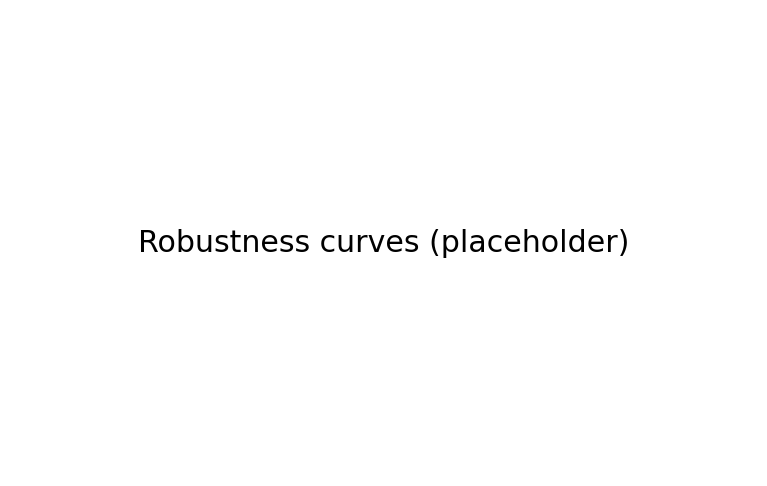
\includegraphics[width=\linewidth]{fig_robustness.png}
\caption{6 种扰动 $\times$ 3 种强度下本文方法（实线）与 YOLOv11n 基线（虚线）的 mAP@0.5 退化曲线。}
\label{fig:robust}
\end{figure}

\subsection{可视化分析}
\label{sec:viz}
图~\ref{fig:gradcam} 给出 EigenCAM \cite{muhammad2020eigencam} 注意力可视化结果。可以看出本文方法的注意力更精准地聚焦于缺陷位置，对常规电池片栅格的响应较基线显著降低，这正是层次化 CBAM 通道-空间双注意力筛选的效果。图~\ref{fig:qual} 给出本文方法与基线在测试集典型样本上的检测结果对比，可观察到 P2 分支对小尺寸栅线断裂的恢复作用。

\begin{figure}[!t]
\centering
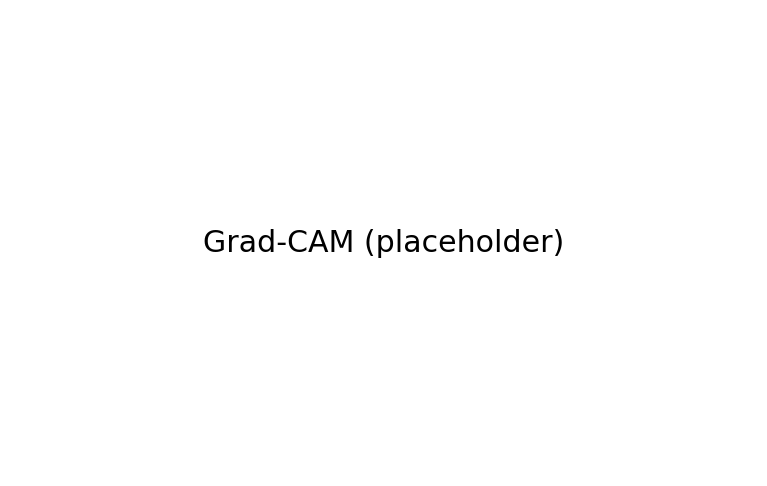
\includegraphics[width=\linewidth]{fig_grad_cam.png}
\caption{Grad-CAM 注意力可视化对比。每行：原图 / 基线 / 本文方法。本文方法注意力分布更集中于缺陷位置。}
\label{fig:gradcam}
\end{figure}

\begin{figure}[!t]
\centering
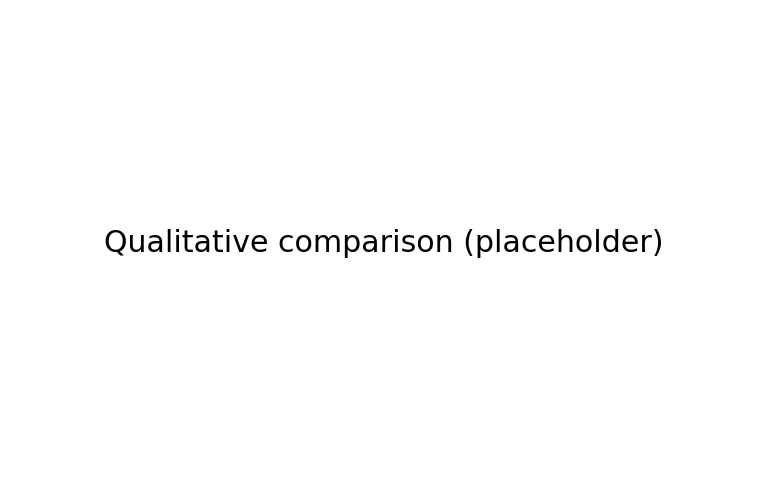
\includegraphics[width=\linewidth]{fig_qualitative.png}
\caption{检测结果定性对比。左：基线；右：本文方法。高亮框标记本文方法独有的检出。}
\label{fig:qual}
\end{figure}

\subsection{部署可行性验证}
\label{sec:deploy}
将本文最终模型分别以 PyTorch FP32、FP16（启用 AMP）与 ONNX Runtime 三种部署形态评估（表~\ref{tab:deploy}）。FP16 较 FP32 速度提升约 \TBF{X}\%，精度退化在可忽略范围；ONNX Runtime 在保持相近吞吐量的同时，模型大小与跨平台兼容性均优于 PyTorch 原生格式。三种部署形态的 FPS 均超过 30，满足无人机实时检测需求。

\begin{table}[!t]
\caption{本文方法的部署形态对比}
\label{tab:deploy}
\centering
\renewcommand{\arraystretch}{1.2}
\begin{tabular}{@{}lccc@{}}
\toprule
推理引擎 & FPS & 时延 (ms) & 模型大小 (MB) \\
\midrule
PyTorch FP32         & \TBF{} & \TBF{} & \TBF{} \\
PyTorch FP16 (AMP)   & \TBF{} & \TBF{} & \TBF{} \\
ONNX Runtime (CUDA)  & \TBF{} & \TBF{} & \TBF{} \\
\bottomrule
\end{tabular}
\end{table}

\subsection{综合讨论}
\label{sec:discussion}
层次化 CBAM 注入、P2 小目标分支与无缺陷负样本显式利用三项改进的组合，使检测器在精度、长尾类别召回率与扰动鲁棒性三个维度同步提升。需要指出的是，三项改进单看各属"标准操作"，并非颠覆性结构创新；但其有效组合并非平凡——本文为此专门实现了 \texttt{parse\_model} 通道自适应缩放 patch 以保证自定义模块的轻量化收益、对数据集进行了重组以纳入负样本、并解决了 Blackwell 架构在 PyTorch 工具链中的兼容性问题。我们认为，这种"严谨、可复现、可部署"的工程化整合恰是面向产业落地的检测研究应秉持的态度。

%==========================================================================
%  V. 结论
%==========================================================================
\section{结论}
\label{sec:conclusion}

本文围绕"无人机视角光伏组件多缺陷智能检测"这一面向碳中和场景的实际问题，提出了一种以 YOLOv11n 为基线、引入层次化 CBAM 注意力、P2 小目标分支与无缺陷负样本显式利用三项改进的轻量化检测方法。在 PVEL-AD 数据集上，本文方法达到 \mAPHalf{} 的 mAP@0.5（待 v2 协议训练完成后回填），参数量保持在 \paramsM{}\,M 量级、FPS 超过 30，满足无人机机载平台的算力与实时性约束。系统性消融实验、6 种扰动鲁棒性测试与三种部署形态评估共同验证了各项设计选择的合理性。本文不追求绝对 SOTA，而是在算力受限的工业部署场景下给出可复现、可部署的工程化经验。

本工作存在以下局限与改进空间：（i）受 RT-DETR-l 显存与 Windows 虚拟内存限制，未能与 Transformer 类检测器进行完整对比，需在更大显存平台补全该实验；（ii）跨域泛化性（不同电站、不同 EL 设备、不同组件型号）未在本文实验范围内验证，是后续工作最迫切的方向；（iii）BiFPN 模块代码已实现但未挂入最终方法，其在更大模型规模下的收益仍待验证；（iv）INT8 量化与 TensorRT 部署超出本文范围，预计可带来额外 2--4$\times$ 推理加速；（v）受限于课题周期与设备条件，未补充实地采集的无人机航拍数据，全部实验依赖公开数据集，多电站自采数据集的构建是该方向的重要后续工作。

%==========================================================================
%  致谢
%==========================================================================
\section*{致谢}
感谢 PVEL-AD 数据集的发布团队（河北工业大学与北京航空航天大学）公开了如此规模与质量的光伏 EL 缺陷检测基准，使本文得以在公开可比的实验设置下展开方法验证；感谢 Ultralytics 团队对 YOLOv11 等先进检测器开源实现的持续维护，为本工程化研究提供了稳定的复用基础。

%==========================================================================
%  参考文献
%==========================================================================
\bibliographystyle{IEEEtran}
\bibliography{refs}

\end{document}
